\documentclass[a4j]{jarticle}

\usepackage{graphicx} 
\usepackage{proc}
\usepackage{mediabb}
\hoffset -2mm

\renewcommand{\baselinestretch}{0.83} % 行間

\title{LLVMコンパイラ基盤を用いたベクトル化コード生成についての検討}
\author{永池 晃太朗}
\mypage{68} % 学科から指定されるページ番号を入力
\begin{document}
\maketitle

\section{はじめに}
画像認識等のデータ並列性の高い処理の高速化にはSIMD命令による処理が効果的である.しかし,SIMD命令による処理は同時演算数を変更する場合,同時に機械語コードを作り直す必要がある.そこで機械語コードの変更なしに同時並列演算数を変更することができる,データ並列処理のためのスケーラブルなベクトル処理機能を備えたベクトル拡張付きRISC-Vを開発された\cite{bib:kimura}.

我々のベクトル拡張付きRISC-Vは,ARMのベクトル拡張であるARM SVE\cite{bib:arm_sve}を参考に組込み向けにRISC-V\cite{bib:risc-v}をベクトル拡張したものである.
これにより,機械語コードが同時演算数に依存しないスケーラブルなベクトル拡張を実現したが,これに対応したコンパイラがない.

この問題に対して,既存のRISC-Vコンパイラをベースとして,我々のベクトル拡張に対応した自動ベクトル化コンパイラを開発する手段を検討する.

%\section{ベクトル拡張付きRISC-V}
%
%我々のベクトル拡張付きRISC-VはRISC-V命令セットで定義されている4つのカスタム命令のためのオペコード領域のうち2つを利用しており,1つをベクトルロード・ストア命令,もう一方をベクトル演算命令とベクトル制御命令に使用している.
%
%ベクトル演算命令は,プレディケート付き演算,プレディケートなし演算命令,即値による演算命令に分けられる.演算命令は,算術論理演算命令,乗除算命令,ベクトルレジスタの各要素の総和を求める命令やアドレス計算の際に用いるインデックスレジスタを生成する命令からなる.プレディケート付き演算命令ではプレディケートレジスタによるベクトルマスク制御を行う.
%
%ベクトル制御命令はプレディケート演算命令とベクトル長操作命令に分けられる.プレディケート演算命令は,プレディケートレジスタ同士の論理演算を行う.これにより柔軟なベクトルマスク制御を行う.ベクトル長操作命令は,スカラレジスタに対しベクトル長を足す等の命令がある.ベクトル制御命令によってスケーラブルなベクトル処理を実現している.

\section{LLVMコンパイラ基盤}
コンパイラの開発にはコンパイラ基盤であるLLVM\cite{bib:llvm}を用いる.
コンパイラ基盤はコンパイラの各機能がモジュール化されており,機能の再利用が行いやすくなっている.
そのため,LLVMで提供されている各種モジュールを利用することで、独自機能部分の実装に集中することができる.
また,LLVMには自動ベクトル化機能が備わっており,入力ソースコードの繰り返し処理をベクトル化されたLLVM IRに変換する.ベクトル化されたLLVM IRでは,処理対象の全データへ演算を行うためにベクトル演算を繰り返した後に余剰分のデータを逐次処理によって演算を行う.
そのLLVM IRからパターンマッチングにより各ターゲットへのベクトル命令への変換などが行われる.
ベクトル拡張付きRISC-VはRISC-Vを拡張しているため,LLVMのRISC-Vコンパイラとしての機能を再利用してコンパイラの開発を行う.

なお,使用するLLVMのバージョンは13.0.0である.

LLVMはソースコードから中間表現であるLLVM IRに変換を行うフロントエンド,LLVM IRからアセンブリコード生成を行うバックエンドからなる.

%\begin{figure}[t]
%    \centering
%    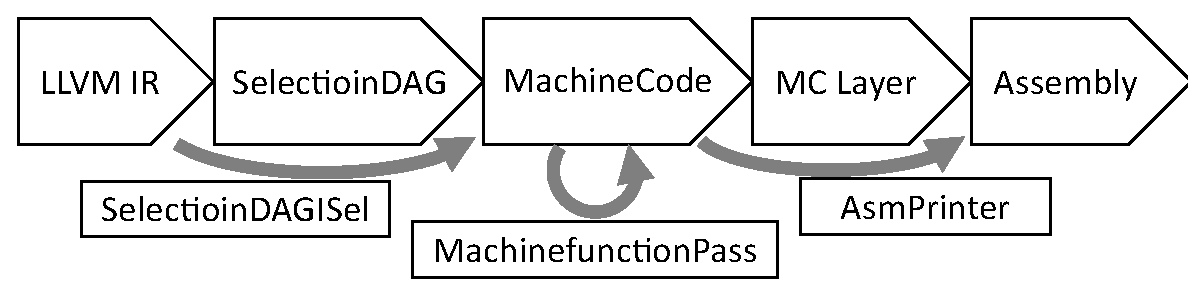
\includegraphics[scale=0.35]{backend_mojideka_2.eps}
%    \caption{コード生成の流れ}
%    \label{fig:backend}
%\end{figure}

%バックエンドにおけるコード生成について,処理の流れとパスを図1に示す.パスとはLLVMにおけるLLVM IR等のコードに対して最適化や変換を行うものである.
%SelectionDAGフェーズではSelectionDAGISelパスによってLLVM IRをDAG (Directed Acyclic Graph)形式へと変換し,DAGのパターンマッチングによるノードの置き換えによる単純化,共通部分削除などの最適化,ターゲット命令への変換の順に行いMachineCode形式を出力する.SelectoinDAGは一つのノードが一つのLLVM IR命令に対応し,命令やデータの依存関係を表すグラフである.
%MachineCode形式はターゲットが使用する実際の命令を持った形式でSSA (Static Single Assignment)形式である.SSA形式では各変数が一度のみ代入される.MachineCodeでは命令のオペランドを仮想レジスタを用いてSSA形式で表現している.MachineCodeはMachinefunctionPassによってSSAベースの最適化を行い,命令への物理レジスタの割当を行う.レジスタの割当を行った後は仮想レジスタによるSSA形式ではなく,オペランドに実際のレジスタを用いた形式となっている.

%MC Layer形式はアセンブリコードに近い形式で,命令とオペランドの情報を持つ.AsmPrinterパスでアセンブリコード,オブジェクトコードを出力する際の中間表現として用いられる.

%以上のLLVMバックエンドでの処理はレジスタ情報,命令フォーマットや命令のニーモニック等の情報に従って行われ,その情報はLLVMにおけるターゲットマシン情報記述のためのドメイン固有言語であるTableGenを用いて記述する.

LLVMのバックエンドではLLVMにおけるターゲットマシン情報記述のためのドメイン固有言語であるTableGenを用いて記述される,レジスタ情報,命令フォーマットや命令のニーモニック等の定義に従ってLLVM IRからアセンブリコードへの変換を行っている.本研究では独自命令生成のためにバックエンドに対して変更を加える.

%LLVMではRISC-VのV拡張用にTableGenによるベクトルレジスタ,ベクトル命令の定義が既に存在している.本研究ではベクトルレジスタはそのまま使用し,ベクトル命令については既存の定義に従った形式でベクトル拡張付きRISC-V命令の定義を行う.


\section{LLVMにおける独自命令の生成機能の実装}

\begin{figure}[b]
    \centering
    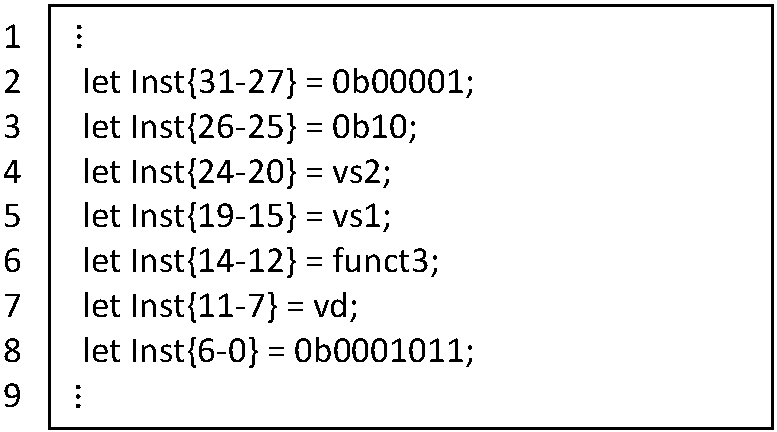
\includegraphics[scale=0.35]{RVInstVVMIQS_min.pdf}
    \caption{命令フォーマットの定義}
    \label{fig:Instruciton_format}
\end{figure}

%ベクトル拡張付きRISC-V命令の定義のために,図1のようなクラスを定義する.クラスRVInstVVMIQSはベクトル要素同士を演算する命令であるベクトル加算等の命令用のフォーマットとして定義する.各命令フォーマットは32bitの命令フィールドを定義している基本クラスRVInstを継承する形で命令によって異なるフォーマットを定義する.

ベクトル拡張付きRISC-V命令の定義のために,各種命令用のフォーマットクラスの定義を行う.図1はベクトル要素同士を演算する命令であるベクトル加算等の命令用のフォーマットの定義である.命令フィールドInstのどの範囲にどの値が入るかを指定している.

\begin{figure}[t]
    \centering
    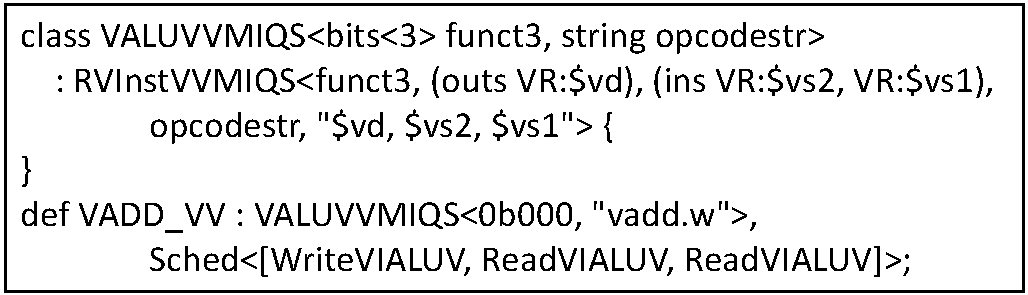
\includegraphics[scale=0.35]{Instruction_min.pdf}
    \caption{命令の定義}
    \label{fig:Instruciton}
\end{figure}

%命令の定義は命令フォーマットのクラスを継承し,エンコードの値やニーモニックを指定して行う.命令の定義を図2に示す.図2のVALUVVMIQSクラスは命令定義の際に同じ定義の繰り返しを防ぐために定義する.同様の入出力レジスタを持つ命令はこのクラスをインスタンス化する際に命令の文字列と命令選択に用いるための12-14ビットの値の指定を行う.

%命令の定義は命令フォーマットクラスを継承した命令定義用クラスをインスタンス化する際に命令文字列や命令選択のための命令フィールドの値の指定して行う.命令定義用のクラスでは入出力レジスタを指定しており,同様の入出力レジスタを持つ命令の定義を行う際に定義の繰り返しを防ぐことができる.

命令の定義は命令定義用クラスをインスタンス化する際に命令文字列や命令選択のための命令フィールドの値の指定して行う.図2にベクトル加算命令の定義を示す.図2のVALUVVMIQSクラスではニーモニックの構成を指定しており,インスタンス化を行う際に命令文字列であるvadd.wと命令選択のための値の指定を行っている.

配列加算のプログラムから実際にアセンブリコードを生成した結果の一部を図1に示す.vadd.wが我々のベクトル拡張命令のベクトル加算命令である.しかし,ロード・ストア命令についてはRISC-VのV拡張の命令のままである.

\begin{figure}[tb]
    \centering
    \vspace{1truemm}
    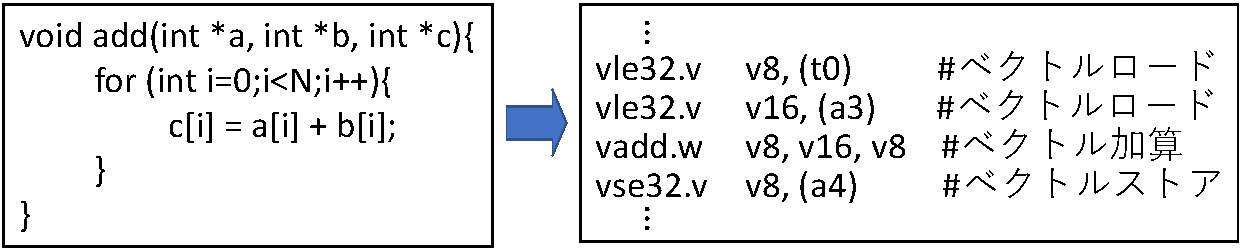
\includegraphics[scale=0.4]{miqs_assembly_yokou.pdf}
    \caption{アセンブリコードの生成}
    \label{fig:assembly}
\end{figure}

現在ベクトル拡張付きRISC-Vのベクトル命令の内,ベクトル演算命令のプレディケートなし,即値による演算命令の実装が完了している.しかし,ロード・ストア命令等が未実装である.それらの命令ではプレディケートレジスタを用いており,新たにプレディケートレジスタの定義を必要とする.また,現在のLLVM IRはベクトル演算の繰り返しと逐次処理によるベクトル処理を行っている.そのため,我々のベクトル拡張のプレディケート付き命令を効果的に利用できない.

\section{おわりに}
本稿では,自動でベクトル化された独自のベクトル拡張付きRISC-V命令アセンブリコードを得るためのLLVMバックエンドの実装を行った.

今後の課題として,ベクトルロード・ストア命令等の未実装の命令生成の実現が挙げられる.
現在実装済みの命令は命令の定義等で実装が可能であった.しかし,未実装の命令については現在のベクトル化されたLLVM IRからの生成が困難であると考えられる.そのため,レジスタの定義に加え,LLVM IRの生成を行うフロントエンドの変更が必要である.


% ------ 参考文献 ------
\begin{thebibliography}{9}
\vspace{-1mm}
\itemsep -1.7pt
{\footnotesize

\bibitem{bib:kimura}
{\small Yoshiki Kimura, et al.:      % 丁寧
%{\small 氏名ほか:             % スペースが足りない場合
\newblock ``Proposal of Scalable Vector Instruction Set for Embedded RISC-V Processor,''
\newblock Proc. 2019 Seventh International Symposium on Computing and Networking Workshops (CANDARW),
\newblock Vol.1,
\newblock pp.435-439,
\newblock 2019.}

\bibitem{bib:arm_sve}
{\small Nigel Stephens, et al.:      % 丁寧
%{\small 氏名ほか:             % スペースが足りない場合
\newblock ``The ARM Scalable Vector Extension,''
\newblock IEEE Micro,
\newblock Vol.37,
\newblock No.2,
\newblock pp.26-39,
\newblock 2017.}

\bibitem{bib:risc-v}
{\small Andrew Waterman, Krste Asanovi:      % 丁寧
%{\small 氏名ほか:             % スペースが足りない場合
\newblock ``The RISC-V Instruction Set Manual Volume I: Unprivileged ISA, Document Version 2.2,''
\newblock 2017.}

\bibitem{bib:llvm}
{\small Chris Lattner, Vikram Adve:      % 丁寧
%{\small 氏名ほか:             % スペースが足りない場合
\newblock ``LLVM: A Compilation Frame-work for Lifelong Program Analysis Transformation,''
\newblock Proc. 2004 International Symposium on Code Generation and Optimization (CGO’04),
\newblock pp.75-86,
\newblock 2004.}

}

\end{thebibliography}

\end{document}

